%% feature_comparisons.tex
%% Author: Leighton Pritchard
%% Copyright: James Hutton Institute 2016
%% Feature comparisons

% FEATURE COMPARISON
\begin{frame}
  \frametitle{Feature comparisons}
    \begin{alertblock}{Feature comparisons}
      Comparisons of the annotated features of one genome with another \\
      ($\ldots$or many others)
      \begin{itemize}
        \item gene features
        \item RNA features
        \item regulatory features
      \end{itemize}
    \end{alertblock}
\end{frame}

% EQUIVALENT FEATURES
\begin{frame}
  \frametitle{Equivalent features}
  \begin{block}{The power of genomics is comparative genomics!}
    \begin{itemize}
      \item Makes catalogues of genome components comparable between organisms
      \item \textcolor{hutton_blue}{Differences, e.g. presence/absence of equivalents may support hypotheses for functional or phenotypic difference}
      \item \textcolor{hutton_green}{Can identify characteristic signals for diagnosis/epidemiology}
      \item \textcolor{hutton_purple}{Can build parts lists and wiring diagrams for systems and synthetic biology}
    \end{itemize}
  \end{block}
  \begin{center}
    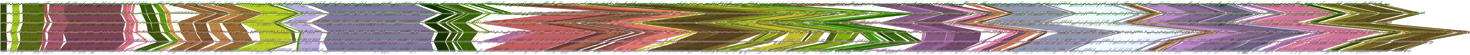
\includegraphics[width=1\textwidth]{images/collinear_zeae}  
  \end{center}  
\end{frame}


% ORTHOLOGUES
\begin{frame}
  \frametitle{Orthologues
  \footnote{\tiny{Nehrt \textit{et al.} (2011) \textit{PLoS Comp. Biol.} \href{http://dx.doi.org/10.1371/journal.pcbi.1002073}{doi:10.1371/journal.pcbi.1002073}}}  
    \footnote{\tiny{Chen \textit{et al.} (2012) \textit{PLoS Comp. Biol.} \href{http://dx.doi.org/10.1371/journal.pcbi.1002784}{doi:10.1371/journal.pcbi.1002784}}}  
  }
  \begin{alertblock}{Orthologs/Orthologues}
    \begin{small}
    ``Homologs that diverged through speciation'' (orig.) \\
    ``Genes/products we think are probably the same thing'' (mod. inform.)
    \end{small}
  \end{alertblock}  
  \begin{center}
    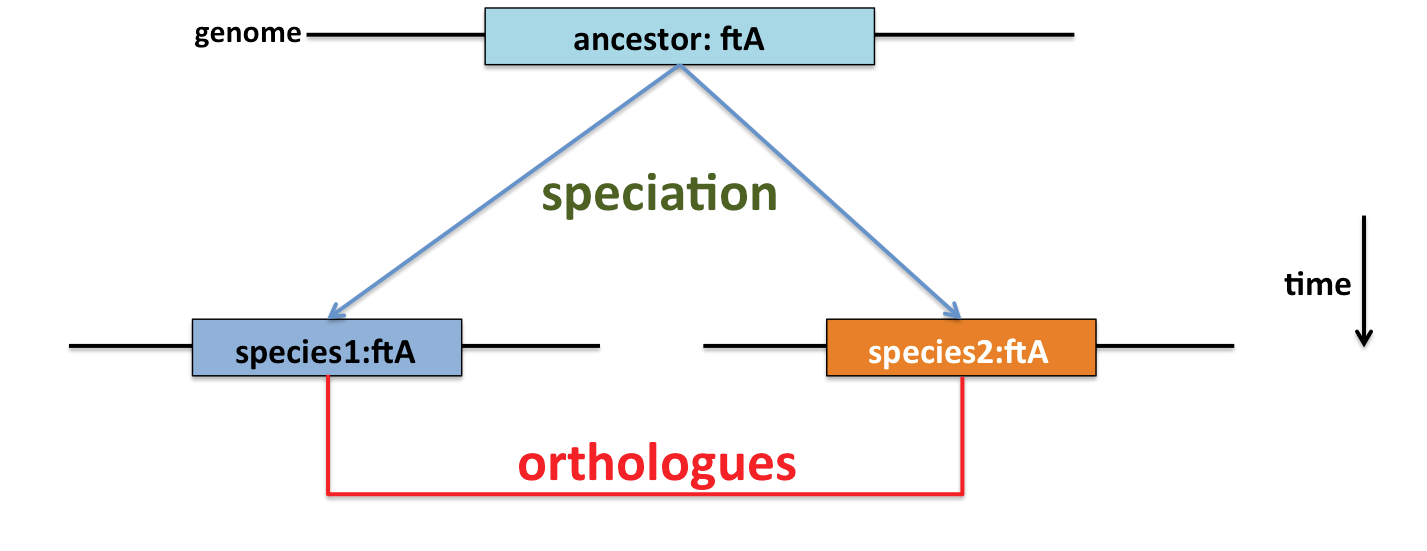
\includegraphics[width=1\textwidth]{images/logues2}  
  \end{center}  
\end{frame}

% ORTHOLOGUES
\begin{frame}
  \frametitle{Why orthologues?
    \footnote{\tiny{Chen and Zhang (2012) \textit{PLoS Comp. Biol.} \href{http://dx.doi.org/10.1371/journal.pcbi.1002784}{doi:10.1371/journal.pcbi.1002784
    }}}  
    \footnote{\tiny{Dessimoz (2011) \textit{Brief. Bioinf.} \href{http://dx.doi.org/10.1093/bib/bbr057}{doi:10.1093/bib/bbr057
    }}}
    \footnote{\tiny{Altenhoff and Dessimoz (2009) \textit{PLoS Comp. Biol.} \textbf{5}:e1000262 \href{http://dx.doi.org/10.1371/journal.pcbi.1000262}{doi:10.1371/journal.pcbi.1000262
    }}}
  }
  \begin{itemize}
    \item Formalise the idea of \textit{corresponding genes} in different organisms.
    \item \textcolor{hutton_blue}{Suggest two relationships:}
      \begin{itemize}
        \item \textcolor{hutton_green}{\textbf{Evolutionary equivalence}}
        \item \textcolor{hutton_purple}{\textbf{Functional equivalence}} (``The Ortholog Conjecture'')
      \end{itemize}
   \end{itemize}
   \begin{alertblock}{The Ortholog Conjecture}
     Without duplication, a gene product is unlikely to change its basic function, because this would lead to loss of the original function, and this would be harmful.
   \end{alertblock}
\end{frame}

% FINDING ORTHOLOGUES
\begin{frame}
  \frametitle{Finding orthologues
    \footnote{\tiny{Salichos and Rokas (2011) \textit{PLoS One} \textbf{6}:e18755 \href{http://dx.doi.org/10.1371/journal.pone.0018755.g006}{doi:10.1371/journal.pone.0018755.g006}}}
  }
  \begin{block}{Which discovery method performs best?}
    \begin{itemize}
      \item Four methods tested against 2,723 curated orthologues from six \textit{Saccharomycetes}: \\
    \textcolor{hutton_green}{RBBH (and cRBH); RSD (and cRSD); MultiParanoid; OrthoMCL} \\
      \item \textcolor{hutton_blue}{Rated by statistical performance metrics: sensitivity, specificity, accuracy, FDR}
    \end{itemize}
  \end{block}
  \textcolor{hutton_purple}{\textbf{cRBH most accurate and specific, with lowest FDR.}}
  \begin{center}
      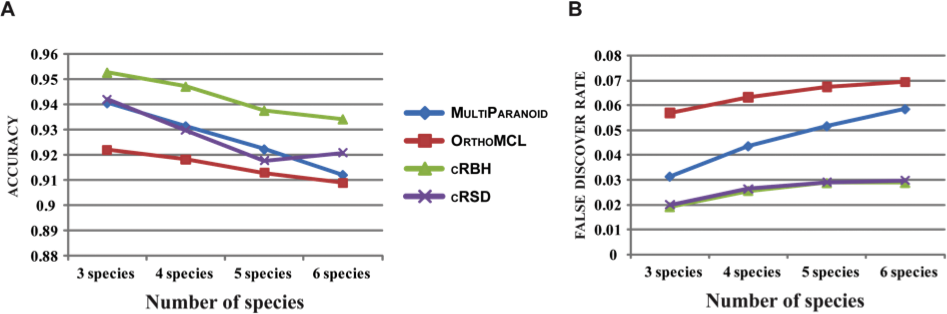
\includegraphics[height=0.25\textheight]{images/salichos_results1} 
      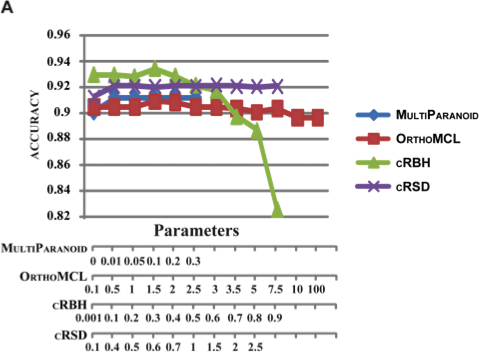
\includegraphics[height=0.25\textheight]{images/salichos_results2}      
  \end{center}
\end{frame}

% EXERCISE
\begin{frame}
  \frametitle{EXERCISE}
  \begin{alertblock}{\url{exercises/02-cds_feature_comparisons.ipynb}}
    \begin{itemize}
      \item RBBH analysis of \textit{Pseudomonas} CDS feature annotations
    \end{itemize}
  \end{alertblock}
  \begin{itemize}
    \item \textcolor{hutton_purple}{\href{http://mybinder.org/repo/widdowquinn/Teaching-EMBL-Plant-Path-Genomics}{MyBinder link}}
  \end{itemize}
\end{frame}

% ONE-WAY BLAST vs RBBH 1
\begin{frame}
  \frametitle{One-way BLAST vs RBBH}   
  \begin{alertblock}{One-way BLAST includes many low-quality hits}
    \begin{center}
      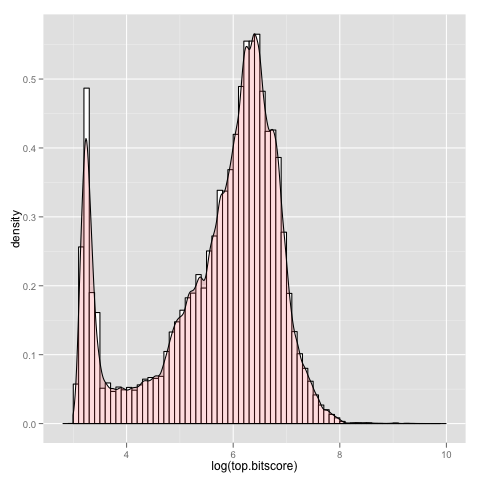
\includegraphics[height=0.33\textheight]{images/rbbh1}
      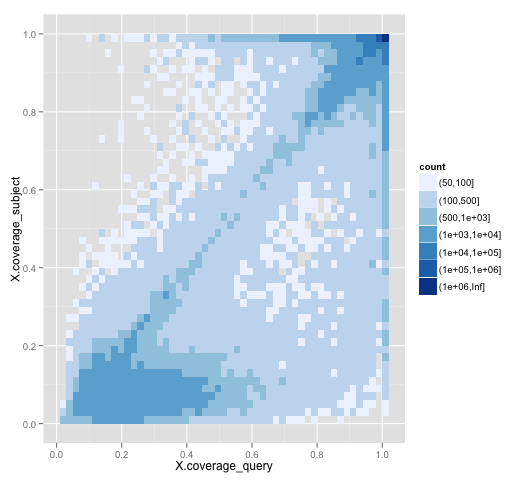
\includegraphics[height=0.33\textheight]{images/rbbh2}
      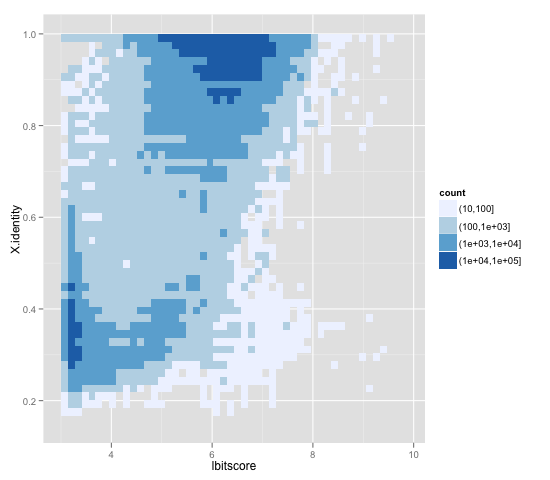
\includegraphics[height=0.33\textheight]{images/rbbh3}
    \end{center}
  \end{alertblock}
\end{frame}

% ONE-WAY BLAST vs RBBH 2
\begin{frame}
  \frametitle{One-way BLAST vs RBBH}   
  \begin{block}{Reciprocal best BLAST removes many low-quality matches}
    \begin{center}
      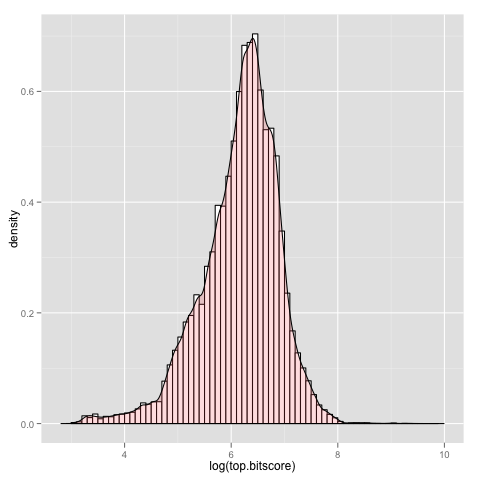
\includegraphics[height=0.33\textheight]{images/rbbh4}
      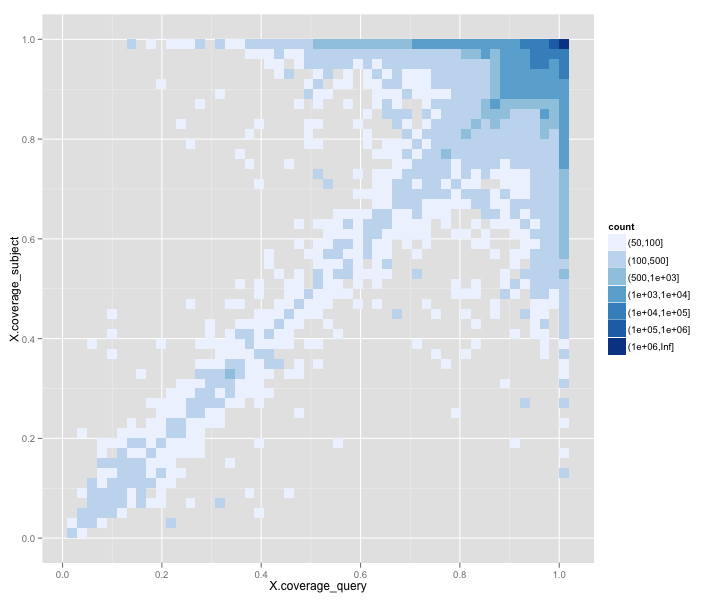
\includegraphics[height=0.33\textheight]{images/rbbh5}
      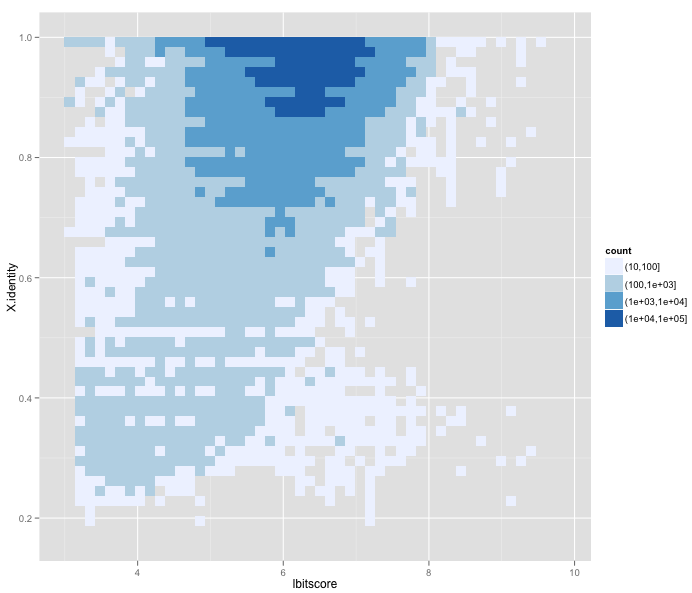
\includegraphics[height=0.33\textheight]{images/rbbh6}
    \end{center}
  \end{block}
\end{frame}

% PANGENOME
\begin{frame}
  \frametitle{The Pangenome}
  \begin{alertblock}{The Core Genome Hypothesis}
    ``The \textit{core genome} is the primary cohesive unit defining a bacterial species''
  \end{alertblock}
  \begin{itemize}
    \item \textcolor{hutton_green}{Once equivalent genes have been identified, those present in all related isolates can be identified: \textbf{\textit{the core genome}}.}
    \item \textcolor{hutton_blue}{The remaining genes are \textbf{\textit{the accessory genome}}, and are expected to mediate function that distinguishes between isolates.}
  \end{itemize}
  \textcolor{hutton_purple}{\href{https://github.com/sanger-pathogens/Roary}{\texttt{Roary}}}: Rapid large-scale prokaryote pan-genome analysis - works on a desktop machine.
\end{frame}

% ACCESSORY GENOMES
\begin{frame}
  \frametitle{Accessory genome
   \footnote{\tiny{Croll and Mcdonald (2012) \textit{PLoS Path.} \textbf{8}:e1002608 \href{http://dx.doi.org/10.1371/journal.ppat.1002608}{doi:10.1371/journal.ppat.1002608}}}
    \footnote{\tiny{Baltrus \textit{et al}. (2011) \textit{PLoS Path.} \textbf{7}:e1002132 \href{http://dx.doi.org/10.1371/journal.ppat.1002132}{doi:10.1371/journal.ppat.1002132}}}  
  }
  \begin{block}{Accessory genomes}
    A cradle for adaptive evolution, particularly for bacterial pathogens, such as \textit{Pseudomonas} spp.
  \end{block}
  \begin{center}
      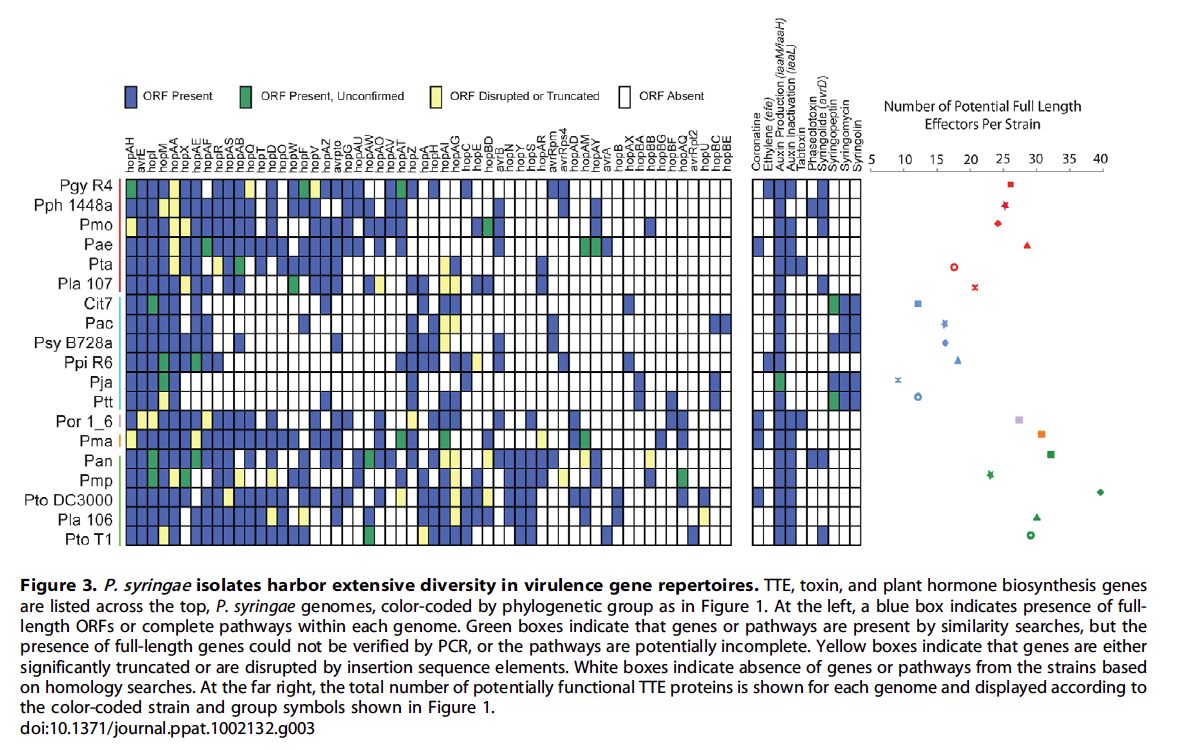
\includegraphics[height=0.45\textheight]{images/pa_virulence} 
  \end{center}
\end{frame}

% WORKSHEET
\begin{frame}
  \frametitle{OPTIONAL WORKSHEET}
  \begin{alertblock}{\url{worksheets/02-prokka_roary.ipynb}}
    \begin{itemize}
      \item Annotation of pathogen genomes with \texttt{Prokka}
      \item Calculation of the \textit{Pantoea agglomerans} pangenome with \texttt{Roary}
    \end{itemize}
  \end{alertblock}
  \begin{itemize}
    \item \textcolor{hutton_purple}{\href{http://mybinder.org/repo/widdowquinn/Teaching-EMBL-Plant-Path-Genomics}{MyBinder link}}
  \end{itemize}
\end{frame}